% !TeX program = xelatex
\ifdefined\pdfminorversion\pdfminorversion=7\fi
\documentclass[final,5p,twocolumn]{elsarticle}

\usepackage{amsmath,amssymb}
\usepackage{booktabs,array}
\usepackage{graphicx}
\usepackage{placeins}
\usepackage{balance}
\usepackage[table]{xcolor}
\definecolor{paperBlue}{HTML}{0072B2}
\definecolor{paperOrange}{HTML}{D55E00}
\definecolor{earlyStageFill}{HTML}{F6E8D6}
\definecolor{lateStageFill}{HTML}{E7EFF5}
\usepackage[colorlinks=true,citecolor=blue,linkcolor=black,urlcolor=black]{hyperref}

\renewcommand{\topfraction}{0.85}
\renewcommand{\textfraction}{0.12}
\renewcommand{\dbltopfraction}{0.85}
\renewcommand{\dblfloatpagefraction}{0.85}
\setlength{\textfloatsep}{8pt plus 2pt minus 2pt}
\setlength{\floatsep}{7pt plus 2pt minus 2pt}
\setlength{\intextsep}{7pt plus 2pt minus 2pt}
\setlength{\dbltextfloatsep}{8pt plus 2pt minus 2pt}
\setlength{\abovecaptionskip}{5pt}
\setlength{\belowcaptionskip}{0pt}
\makeatletter
\renewcommand\section{\@startsection{section}{1}{\z@}%
  {-2.2ex plus -0.5ex minus -0.2ex}{0.8ex plus 0.2ex}%
  {\normalfont\large\bfseries\raggedright}}
\renewcommand\subsection{\@startsection{subsection}{2}{\z@}%
  {-1.6ex plus -0.4ex minus -0.2ex}{0.6ex plus 0.2ex}%
  {\normalfont\normalsize\bfseries\raggedright}}
\renewcommand\subsubsection{\@startsection{subsubsection}{3}{\z@}%
  {-1.2ex plus -0.3ex minus -0.1ex}{0.4ex plus 0.1ex}%
  {\normalfont\small\bfseries\raggedright}}
\setlength{\@fptop}{0pt}
\setlength{\@fpsep}{10pt plus 2pt}
\setlength{\@fpbot}{0pt plus 1fil}
\setlength{\@dblfptop}{0pt}
\setlength{\@dblfpsep}{10pt plus 2pt}
\setlength{\@dblfpbot}{0pt plus 1fil}
\makeatother

\journal{}

\def\FigureAssetRoot{figure_package}
% Native LaTeX captions; the elsarticle main-caption formatter is preserved.
\usepackage[caption=false,font=footnotesize,position=bottom,labelformat=parens,labelsep=space]{subfig}
\providecommand{\FigureAssetRoot}{.}
\providecolor{paperBlue}{HTML}{0072B2}
\providecolor{paperOrange}{HTML}{D55E00}
\definecolor{figAll}{HTML}{252C31}
\definecolor{figGray}{HTML}{7B858C}
\definecolor{figGreen}{HTML}{009E73}
\newcommand{\ESPanel}[3]{\begin{minipage}[t]{#1}\vspace{0pt}\centering\subfloat[#3]{\includegraphics[width=\linewidth]{\FigureAssetRoot/#2}}\end{minipage}}


\begin{document}
\raggedbottom
\begin{frontmatter}
\title{\bfseries Human Variation and Structural Consensus in Panoramic Room Layout Annotation: The Roles of Group Size and Composition}
\author{}
\begin{abstract}
Reliable panoramic room layout annotations are essential for training and evaluating scene-understanding models. Yet reference layouts can omit visible structures, and annotators can disagree on spatial extent, wall turns and boundary placement. These inconsistencies can introduce noisy supervision and make model evaluation depend on the chosen annotation. We present a framework for characterizing annotation differences and constructing collective layouts, linking geometric measurement, structural aggregation and target-space definition. A geometric quality measure, $Q$, captures extent, boundary, direction and height discrepancies, while paired-corner structural consensus combines support and upper--lower observations into a connected layout. We define doorway-boundary viewpoints as a distinct annotation setting: a camera beneath a doorframe exposes adjoining spaces, requiring an explicit choice of enclosure and closure boundary.

Using 6,512 Manual annotations from 60 people across 206 panoramas in 22 buildings, we investigate group size through Monte Carlo sampling and composition through controlled member replacements. Across 171 panoramas, increasing teams from 3 to 6 people raises mean $Q$ by 4.74 points. Expanding from 20 to 30 raises the mean by only 0.50 points but improves the within-image 10th percentile by 2.85 points. In 14-person teams, replacing 7 members with annotators from a more turn-retaining class raises mean $Q$ by 6.19 points, with gains on 77 of 83 panoramas. Across views of the same room, annotators exhibit recurring tendencies to retain or simplify structure, alongside viewpoint-dependent corner choices. Together, these findings guide team organization, target definition and targeted re-annotation to produce higher-quality layout datasets, providing stronger supervision and more reliable benchmarks for scene-understanding models.
\end{abstract}
\begin{keyword}
Panoramic room layout \sep Annotation quality \sep Annotation aggregation \sep Inter-annotator variation \sep Group size \sep Annotator composition
\end{keyword}
\end{frontmatter}

\section{Introduction}

Training and evaluating indoor panorama interpretation systems requires reliable 3D room layout references. A reference specifies both the space to represent and the geometry of its boundaries. Our review of MatterportLayout references for Matterport3D panoramas \cite{chang2017matterport3d,zou2021manhattan} found ambiguities around openings and hidden extensions, together with geometric errors within the selected rooms, including omitted fireplace projections and visible wall turns. Reliable annotation therefore requires an explicit target and careful tracing of the structures that define it.

Even with the target fixed, human annotators produce different layouts. One annotator bridges a fireplace with a straight wall while another traces its recessed sides (Figure~\ref{fig:individual-fireplace}). Annotators who retain the same turn also place its upper and lower endpoints at different positions. These differences raise a connected set of questions: which individual choices recur, how do they enter a collective layout, and how does the result change when we add or replace people? Answering them requires following both structural support and boundary geometry through the aggregation process.

\begin{figure}[t]
\centering
\setcounter{subfigure}{0}
\begin{minipage}{86mm}
\centering
\begin{minipage}[t]{.36\linewidth}
\vspace{0pt}\centering
\ESPanel{\linewidth}{panels/fig01/a.pdf}{Panorama}
\par\vspace{3pt}
\ESPanel{\linewidth}{panels/fig01/b.pdf}{Room context}
\end{minipage}%
\hfill%
\ESPanel{.326\linewidth}{panels/fig01/c.pdf}{A29 (4 corners)}%
\hfill%
\ESPanel{.2840275\linewidth}{panels/fig01/d.pdf}{A59 (8 corners)}

\par\vspace{2pt}
\includegraphics[width=.66\linewidth]{\FigureAssetRoot/panels/fig01/legend.pdf}
\par\vspace{2pt}

\end{minipage}
\caption{(a) Panorama 7y3sRwLe3Va-19 and (b) room context. (c) A29 bridges the fireplace with four corners; (d) A59 traces its sides with eight. The footprints share a scale, with the reference dashed; the lower row shows the room context and the three-dimensional layouts reconstructed from each annotation.}
\label{fig:individual-fireplace}
\end{figure}


Recent work clarifies alternative layout targets and improves reference construction \cite{c2ref06,dong2024panocontext,kanayama2025tof360}, while annotation research models worker differences and aggregates complex responses \cite{c2ref07,c2ref17}. For panoramic layouts, structural choices and positional variation are coupled: omitting a shallow recess changes the wall sequence with little change in floor coverage, whereas shifting a shared upper endpoint changes local wall height without changing the corner count. A study of collective layout quality must measure these differences and preserve their connection to the people who supplied the observations.

We propose a framework for understanding annotation differences and constructing collective panoramic room layouts. It links target-space definition, geometric quality measurement and paired-corner structural consensus: defining which enclosure to annotate, measuring geometric discrepancies, and combining observations into a shared layout. Controlled comparisons vary team size, class composition, specific members and retained teammates, while same-room comparisons examine which individual choices recur across viewpoints. Together, these components connect annotation choices to collective geometry and support reference review and team organization. Our contributions are fourfold:

\textbf{Geometric quality measurement.} We introduce $Q$ to measure spatial extent, boundary placement, orthogonal regularity, and global and local height discrepancies. It detects local height distortions obscured by mean-height prism overlap while remaining invariant to collinear subdivisions that preserve wall geometry. Controlled geometric tests and real annotation defect reports establish the interpretation of these measurements.

\textbf{Paired-corner structural consensus.} We develop a method for constructing a shared layout from multiple annotators' paired upper--lower corner observations. It aligns variable-length cyclic wall sequences, retains turns through distinct-person support, and aggregates their upper and lower positions into a connected layout. This carries shared structural observations and local upper boundaries beyond the floor coverage represented by region voting.

\textbf{Doorway-boundary target definition.} We define doorway-boundary viewpoints, where a camera beneath a doorframe exposes adjoining spaces. Choosing either room or their combined space changes the target enclosure and its closure boundary. Making these alternatives explicit separates target choice from geometric accuracy and provides a basis for annotating and evaluating this distinct scene setting.

\textbf{Group-size and composition effects on collective layouts.} We show that adding annotators affects mean quality and the lower tail differently, while class proportions, specific members and retained teammates shape collective structure and geometry. Controlled within-class and cross-class replacements distinguish the magnitude of change from its direction; teams with identical class proportions can produce different layouts, and retained teammates can reverse the effect of the same replacement. Same-room comparisons further identify recurring structural habits alongside viewpoint-dependent corner choices. These findings inform team composition and targeted review beyond simply increasing the number of annotators.

\section{Background and Related Work}

\subsection{Layout targets, representations and measurement}
Panoramic layout estimation represents indoor enclosures through wall turns and their ceiling and floor boundaries \cite{c2ref01,horizon2019}. MatterportLayout and ZInD supply references across diverse indoor scenes \cite{zou2021manhattan,cruz2021zind}, but choosing the enclosed space remains part of the annotation task. Bi-Layout distinguishes layouts that stop at openings from layouts that extend into visible adjoining spaces \cite{c2ref06}. Recent efforts have also scrutinized reference fidelity: ReplicaPano combines and refines annotations across viewpoints of the same room to construct a consistent layout \cite{dong2024panocontext}, while ToF-360 uses building geometry to annotate occluded elements and documents a missing wall plane in a MatterportLayout example \cite{kanayama2025tof360}. These studies show why a reliable reference depends on both the intended enclosure and the evidence used to trace it. A camera beneath a shared doorframe makes this distinction particularly consequential: either adjoining room or their combined space may be selected, with different closure boundaries. The doorway-boundary setting makes these target choices explicit before individual and collective layouts are compared.

Layout evaluation uses overlap, corner, pixel and depth measures under different representations and benchmark protocols \cite{horizon2019,horizoneval,zou2021manhattan}. For freely marked upper endpoints, reducing the layout to a mean-height prism can conceal opposing local height errors. Likewise, omitting a shallow recess may substantially change the wall sequence while barely changing floor overlap. These cases motivate measuring the geometry behind a score. The proposed $Q$ combines extent, boundary placement, orthogonal regularity and global and local height measurements, retaining interpretable components that can be examined alongside structural differences.

\subsection{Annotator differences and spatial aggregation}
Repeated-labeling models account for worker-specific error rates, multidimensional expertise and item difficulty \cite{c2ref13,c2ref08,c2ref09}, and redundant annotations can improve label accuracy \cite{c2ref19,c2ref25}. Other approaches examine the structure of disagreement itself. Studies of divergent interpretations identify annotator groups with recurring labeling patterns \cite{c2ref07}, while CrowdTruth relates disagreement to workers, items and labels \cite{c2ref11}. Research on textual inference and human label variation likewise treats differing judgments as information about the task and its interpretations \cite{c2ref10,plank2022variation}. In panoramic annotation, such differences appear both in which wall turns people retain and in where they place shared corners. Repeated simplification of recesses or retention of short walls therefore provides information about individual annotation patterns as well as geometric accuracy.

Spatial aggregation methods differ in the units they combine. STAPLE estimates segmentation truth and annotator performance from pixel labels \cite{c2ref14}, whereas boundary-based segmentation aggregation forms planar cells from overlapping submitted polygons \cite{lee2018}. A general annotation-aggregation model combines distance-based selection, decomposition, merging and object matching across simple, complex and multi-object tasks \cite{c2ref17}. For panoramic layouts, the aggregation unit must also preserve the cyclic wall sequence and the relationship between upper and lower endpoints, even when annotators mark different numbers of turns. Paired-corner structural consensus combines these observations through cyclic matching, distinct-person support and periodic position aggregation. This representation makes it possible to trace both supported turns and their upper boundaries into the output, complementing the floor coverage captured by BEV region voting.

The choice of aggregation unit also makes member contributions observable. Replacing an annotator can add support for a missed turn, weaken support for a recess or shift a shared boundary, distinctions that average worker or class quality alone cannot describe. Separating class proportions from specific membership, and comparing the same exchanged members against different retained teammates, reveals how individual patterns interact in the collective layout.

\subsection{Task conditions and cross-view histories}
Interactive layout workflows combine proposed geometry with human editing. PanoAnnotator supports initialization, refinement and geometric constraints \cite{pano2018}; ZInD combines automated layout proposals and floor-plan assembly with human correction and verification \cite{cruz2021zind}. In clinical text annotation, fully pre-populated suggestions reduced experts' initiative to create additional annotations \cite{levy2021suggestions}. Annotation guidelines and familiarity with the data also shape task performance \cite{c2ref21,c2ref12}. These findings motivate distinguishing the presence of an edit from the correction of a defect. Manual and Semi submissions provide complementary observations of layouts drawn from scratch and responses to initialized geometry.

Multi-view layout methods use complementary observations of the same room: PSMNet merges layout information across viewpoints, and 360-MLC uses cross-view consistency for self-training and parameter selection \cite{c2ref23,c2ref24}. Shared room geometry offers a corresponding opportunity to study human annotation: changing the viewpoint changes visibility while retaining the room being described. The central questions are whether an annotator repeatedly retains or simplifies structure, which local corner choices change, and whether a specified member replacement has a similar effect across views. Structural histories and quality histories provide distinct evidence about what can transfer between these observations.

\section{Research Approach and Study Design}
Figure~\ref{fig:study-design} summarizes how independent annotations enter geometric quality measurement, structural consensus and the four empirical comparisons.

\begin{figure*}[t]
\centering
\setcounter{subfigure}{0}
\begin{minipage}{145mm}
\centering
\includegraphics[width=\linewidth]{\FigureAssetRoot/panels/fig02/a.pdf}
\end{minipage}
\caption{Overview of the study. Independent Manual and Semi submissions provide spatial observations; geometric quality measurement and structural consensus support controlled comparisons of individuals, group size, team composition and cross-view patterns.}
\label{fig:study-design}
\end{figure*}

\label{sec:methods}

The framework connects three operations: defining the enclosure to be annotated, measuring each submitted layout, and combining observations into a collective layout. Controlled team comparisons then isolate changes due to team size and membership. Each submission is an ordered ring of upper--lower corner pairs. The lower endpoint determines a floor-level wall junction; the upper endpoint determines its local height. Small endpoint shifts can change the reconstructed wall substantially (Figure~\ref{fig:observed-geometry}), so both methods retain the geometry carried by these observations.

\begin{figure}[t]
\centering
\setcounter{subfigure}{0}
\begin{minipage}{82mm}
\centering
\ESPanel{.64\linewidth}{panels/fig03/a.pdf}{Panorama}%
\hfill%
\ESPanel{.33\linewidth}{panels/fig03/b.pdf}{Floor corner}

\par\vspace{3pt}
\ESPanel{.34\linewidth}{panels/fig03/c.pdf}{Full BEV}%
\hfill%
\ESPanel{.476\linewidth}{panels/fig03/d.pdf}{3D overlay}

\par\vspace{2pt}
\includegraphics[width=.64\linewidth]{\FigureAssetRoot/panels/fig03/legend.pdf}
\par\vspace{2pt}

\end{minipage}
\caption{Image observations and reconstructed geometry. A floor endpoint displacement from P to P' changes the footprint and the corresponding wall in three dimensions. The assessed layout is blue and the reference is dashed gray.}
\label{fig:observed-geometry}
\end{figure}


\subsection{Geometric quality measurement}
\label{sec:quality}

A layout can cover the correct floor area while distorting the ceiling, or have orthogonal walls around the wrong enclosure. We introduce $Q$ to measure these differences through floor overlap, boundary displacement, internal direction, mean height and local height. Figure~\ref{fig:quality-components} shows two controlled changes and their resulting scores. Geometric responses and human judgments are evaluated in Section~\ref{sec:q-validation}.

\begin{figure*}[t]
\centering
\setcounter{subfigure}{0}
\begin{minipage}{\textwidth}
\centering
\ESPanel{.24\linewidth}{panels/fig04/fig04_a.pdf}{Boundary shift: 0.4 m}%
\hfill%
\ESPanel{.24\linewidth}{panels/fig04/fig04_b.pdf}{Boundary shift: 1.2 m}%
\hfill%
\ESPanel{.24\linewidth}{panels/fig04/fig04_c.pdf}{Local height shift: $\pm 0.3$ m}%
\hfill%
\ESPanel{.24\linewidth}{panels/fig04/fig04_d.pdf}{Local height shift: $\pm 1.2$ m}

\par\vspace{2pt}
\includegraphics[width=.82\linewidth]{\FigureAssetRoot/panels/fig04/fig04_legend.pdf}
\par\vspace{2pt}

\end{minipage}
\caption{Controlled examples show how geometric changes affect Q. The reference room has a $4\times4$ m footprint, a 3 m wall height and a 1.6 m camera height. (a--b) Moving one floor boundary inward reduces overlap and increases boundary distance; hatched regions mark omitted floor area. (c--d) Opposing upper-boundary shifts preserve the footprint and perimeter-mean height while increasing local height error. Blue and orange show the smaller and larger changes; dashed gray denotes the reference. Measurements and Q are computed from the displayed geometry.}
\label{fig:quality-components}
\end{figure*}


Let $P$ and $R$ denote a layout and its assigned reference, reconstructed in camera-height units with floor plane $y=-1$. Each upper--lower pair is horizontally aligned to the midpoint of its shorter arc, retaining both vertical coordinates and hence its local wall height (Supplement B5). For floor polygons $A_P$ and $A_R$, overlap is $I=|A_P\cap A_R|/|A_P\cup A_R|$. Boundary distance $S_b$, in degrees, symmetrically averages the nearest angular distance from uniformly spaced samples on each spherical floor contour to the other continuous boundary.

Internal orthogonal regularity depends on $P$ itself. For floor edges with lengths $\ell_e$ and plan-view orientations $\alpha_e$, we fit the orthogonal axis pair that minimizes the length-weighted residual:
\begin{equation}
 D_{\mathrm{dir}}(P)=\min_{0\leq\phi<90^\circ}
 \sqrt{\frac{\sum_e\ell_e\operatorname{wrap}_{90^\circ}(\alpha_e-\phi)^2}{\sum_e\ell_e}},
 \label{eq:direction}
\end{equation}
where $\operatorname{wrap}_{90^\circ}$ maps deviations into $[-45^\circ,45^\circ)$.

Heights are interpolated linearly along floor edges. For cyclic corner heights $h_i$, the perimeter-weighted mean is
\begin{equation}
 \mu_P=\frac{\sum_i\ell_i(h_i+h_{i+1})}{2\sum_i\ell_i}.
 \label{eq:perimeter-height}
\end{equation}
Mean-height error is $H_m=|\mu_P-\mu_R|/\mu_R$. Local-height error $H_c$ is the symmetric root-mean-square difference between mean-centered height profiles, normalized by $\mu_R$. Each perimeter sample is compared with the nearest floor position on the other layout; distance ties use the largest squared height residual. Integrating along the perimeter makes both height measurements invariant to subdividing an unchanged straight wall with collinear points (exact expressions in Supplement C18).

For a valid layout with positive overlap, the measurements give
\begin{align}
 F&=\left(\frac1I-1\right)+\frac{S_b^2}{32}, &
 L_d&=1.5\frac{D_{\mathrm{dir}}^2}{D_{\mathrm{dir}}^2+8^2},\label{eq:floor-loss}\\
 L_m&=\left(\frac{H_m}{0.8}\right)^2, &
 L_c&=\left(\frac{H_c}{0.25}\right)^2,\label{eq:height-loss}
\end{align}
and
\begin{equation}
 Q(P,R)=\frac{100}{1+\sqrt{F^2+L_d^2}+L_m+L_c}.\label{eq:quality}
\end{equation}
If floor overlap is the only discrepancy, $Q=100I$. Scorable layouts have a simple, nondegenerate floor polygon, at least three corner pairs, positive wall heights and valid boundary projections. Valid polygons with zero overlap receive $Q=0$; incomplete or degenerate outputs remain unscorable and enter the completion-rate analysis (Supplement C15).

\subsection{Structural consensus from paired corner observations}
\label{sec:consensus}

A shallow recess may occupy little floor area yet introduce two wall turns that some people retain and others bridge over. Paired-corner structural consensus makes these choices explicit: it identifies corresponding pairs, counts their distinct supporters, aggregates their positions, and connects the retained pairs into a layout. Figure~\ref{fig:consensus-steps} follows actual observations into their resulting boundary and three-dimensional geometry.

\begin{figure*}[t]
\centering
\setcounter{subfigure}{0}
\begin{minipage}{170mm}
\centering
\ESPanel{.322\linewidth}{panels/fig06/a_upper_evidence.pdf}{Upper observations}%
\hfill%
\ESPanel{.322\linewidth}{panels/fig06/b_lower_evidence.pdf}{Lower observations}%
\hfill%
\ESPanel{.322\linewidth}{panels/fig06/c_actual_layout.pdf}{Connected 3D layout}
\par\vspace{2pt}
\includegraphics[width=\linewidth]{\FigureAssetRoot/panels/fig06/legend.pdf}
\par
\end{minipage}
\caption{Paired observations form the recessed wall in jtcxE69GiFV-13, Team 2. (a) Eight upper observations per turn, their medians and the resulting upper boundary. (b) The same supporters' lower observations projected to the floor, with individual wall traces in gray and consensus in purple. (c) Complete six-corner layout and enlarged upper-wall detail, using the same coordinates and view; rear edges are dashed. A and B identify the same turns throughout. Each corner retains its local height; $h$ denotes camera height.}
\label{fig:consensus-steps}
\end{figure*}


An observation $a_{wj}=(p^t_{wj},p^b_{wj})$ contains annotator $w$'s upper and lower endpoints. Matching cost is their mean spherical angular distance, $c(a,b)=[\theta(p_a^t,p_b^t)+\theta(p_a^b,p_b^b)]/2$. Dynamic programming over cyclic starting points and both traversal directions gives partial one-to-one matches while allowing unmatched corners:
\begin{equation}
 \pi_{uv}^{*}=\underset{\pi\in\Pi_{uv}}{\arg\min}
 \left[\sum_{(a,b)\in\pi}c(a,b)
 +g\bigl(n_u^{\mathrm{skip}}+n_v^{\mathrm{skip}}\bigr)\right],
 \label{eq:cyclic-match}
\end{equation}
where $n_w^{\mathrm{skip}}$ counts unmatched observations and $g$ is their per-observation skip penalty. Complete-linkage clustering partitions the pairwise matches into disjoint corner clusters $G$, requiring pairwise support throughout each cluster and at most one observation per annotator.

For team $S$, a cluster is retained when at least half the team supports it:
\begin{equation}
 z(G)=\mathrm{1}[2s(G)\geq |S|],
 \label{eq:mv50}
\end{equation}
where $s(G)$ counts distinct supporting annotators. This MV50 rule includes exact-half support. Only supporters contribute to the retained corner's coordinates, with equal weight. Horizontal positions are unwrapped around an observed anchor and aggregated by the median; upper and lower elevations use separate medians. The retained pairs are connected in cyclic wall order and checked for geometric validity (Supplements C15--C16, C18). Section~\ref{sec:method-validation} examines how support and upper endpoints enter the output.

\section{Evaluation Protocol}
\label{sec:study-design}

The protocol recombines independent submissions while fixing the image, task condition and target reference. It separates the effect of adding people from changes in profile composition, individual membership and retained background (Table~\ref{tab:principal-analysis-sets}). Cross-view and doorway comparisons then examine changes in visual evidence and enclosure choice.

\subsection{Task, participants and reference targets}

Participants marked the walls enclosing the camera, including architectural recesses, while ignoring movable furniture and decoration. The main task assumes vertical walls along two orthogonal plan-view axes, a closed single-level footprint, and single floor and ceiling planes. Openings are closed at identifiable structural divisions such as doorframes or paired wall ends. Doorway-boundary viewpoints place the camera beneath a doorframe and expose adjoining enclosures. These cases require an explicit target and are analyzed separately from ordinary rooms; oblique walls, sloped ceilings and split levels form an out-of-scope (OOS) cohort.

Participants were recruited from university cohorts and Upwork, received an average of USD~0.50 per panorama, and consented to duration recording and research use. After instruction and practice, \textit{Manual} annotators placed and ordered upper--lower pairs from scratch using an interactive 3D preview. \textit{Semi} annotators edited HoHoNet predictions \cite{hohonet2021} or six controlled-defect initializations on separate panoramas. The main collection contains 6,512 Manual submissions from 60 people on 206 panoramas in 22 buildings and 960 Semi submissions from 59 people on 37 panoramas in 12 buildings; 57 of the 62 total participants contributed to both modes (Supplements B1, C12, C20).

Before the study, three experts with experience annotating 100 panoramas and detailed knowledge of Manhattan layouts reviewed MatterportLayout references \cite{chang2017matterport3d,zou2021manhattan}, resolved target rules, corrected geometric errors, and catalogued natural Semi initialization defects. Reference corner counts, self-occlusion and expert inspection define easy, moderate and difficult tiers. Experts screened doorway responses for insufficient points or uninterpretable enclosures while blinded to $Q$. The fixed 17-image screening comparison retains the same whole-space reference before and after screening; separate target-assigned pools address enclosure choice (Supplements C15, C17, C20).

\subsection{Controlled team comparisons}

For RQ2, Monte Carlo sampling with 256 uniformly random entry orders per eligible pool form nested teams of 3--30 people on a fixed panel of 171 panoramas. For RQ3, profiles are derived from each person's history outside the target building. Structural classes C1--C3 represent simplifying, typical and turn-retaining tendencies. Their features cover corner counts, short edges, near-collinear vertices and reference matches. Within each training fold, robust scaling, domain-wise PCA and domain balancing precede Ward clustering; classes are ordered by difficult-image turns and short edges, then overall turns. Effective turns exceed $5^\circ$; short edges occupy less than 4\% of the perimeter with endpoint turns of at least $15^\circ$. Consensus-response (R1--R2) profiles summarize historical effects on group geometry; joint profiles (J1--J4) combine structural, geometric, historical-quality and duration features (Supplements C6--C9).

\begin{table*}[t]
\centering\small
\caption{Principal controlled comparisons. The image and target are fixed except where viewpoint or target is the studied factor. Supports overlap; Supplement C20 reports full coverage.}
\label{tab:principal-analysis-sets}\label{tab:analysis-support}
\setlength{\tabcolsep}{5pt}\renewcommand{\arraystretch}{1.12}
\begin{tabular}{@{}>{\raggedright\arraybackslash}p{.19\textwidth}>{\raggedright\arraybackslash}p{.31\textwidth}>{\raggedright\arraybackslash}p{.44\textwidth}@{}}
\toprule
Comparison & Support & Controlled change and outcome\\
\midrule
Group size & 171 images; 22 buildings; 256 orders/image & Add people; quality distribution and completion\\
Shared structure & 70 Manual teams; 24 images; 14 buildings & Same submissions; floor coverage, turns and upper boundaries\\
Matched replacement & 69 images; 20 buildings; 146/147 scorable events & Replace 7/14 members; excess magnitude and direction\\
Retained background & 276 blocks; 7 images & Same exchange, different retained members; direction\\
Cross-view structure & 128 view pairs; 65 images; 13 buildings & Same and different people across room views; repetition and transfer\\
Doorway screening & 17 images; 9 buildings; 584/439 responses before/after & Screen responses against the same whole-space reference\\
\bottomrule
\end{tabular}
\end{table*}

A direct replacement compares $A=D\cup X$ with $C=D\cup Z$, retaining members $D$ while exchanging equal-sized blocks $X$ and $Z$. The matched A--B--C design adds $B=D\cup Y$: $X$ and $Y$ share a profile, $Z$ has a contrasting profile, and $D,X,Y,Z$ are mutually disjoint. It separates excess change magnitude from direction:
\begin{align}
G_S&=\frac{|Q_C-Q_A|+|Q_C-Q_B|}{2}-|Q_B-Q_A|,\label{eq:symmetric-excess}\\
\Delta_{CB}&=Q_C-Q_B.\label{eq:directional-change}
\end{align}
Effects are averaged over valid exchanges and backgrounds within each image, then equally over images. Fixed-size profile ratios and whole-profile mixtures test composition; holding $(X,Z)$ fixed while changing $D$ tests background dependence (Supplement C17).

\subsection{Method assessment and outcome measures}

The $Q$ form and scales were fixed using controlled geometric perturbations before human validation and team analysis. Measurements use 2,048 boundary and 4,096 height samples per direction. Consensus uses $g=7.5^\circ$ per skipped observation to accommodate within-corner variation while distinguishing nearby turns. Supplement C16 records these settings and the existing score-scale sensitivity checks.

For human validation, two Manual annotations were randomly sampled from each of 30 panoramas in 17 buildings: nine easy, nine moderate, nine difficult and three doorway images. Eight randomly invited annotators graded them as good, medium or poor and marked visible defects using randomized displays of panorama overlays, shared-scale footprints and 3D views. Shared-team assessment compares the same teams using paired-corner consensus and BEV region voting, which retains planar cells covered by at least half the team \cite{lee2018}.

Team outcomes are mean $Q$, within-image P10, between-team standard deviation, and complete-and-evaluable rate. Quality comparisons use scorable outputs; completion counts all attempts. For group-size curves, 2,000 bootstrap resamples of entry trajectories estimate Monte Carlo precision, while 2,000 building resamples describe variation across the 22 buildings with the observed annotators retained.

Offline selection and stopping use recorded annotation person-time. Quality-and-time selection exchanges members of a historical-$Q$ team for faster people within a two-point historical-quality tolerance. Source-history stopping uses other views to select the earliest team size within two points of their expected peak, continuing to obtain a complete polygon. It is compared with fixed seven-person teams and a three-step corner-count stability rule; source-history acquisition is included in project labor (Section~\ref{sec:labor-history}, Supplements C8--C9, C20).

\section{Results}
\label{sec:results}
\subsection{Individual Expression Under Image and Initialization Conditions}
\label{sec:individual}

Annotators differ in both retained structure and boundary position. The fireplace example contrasts an eight-turn recess with a four-turn enclosure (Figure~\ref{fig:individual-fireplace}); even annotators retaining the same turns place their endpoints differently. The out-of-building profiles distinguish simplifying (C1), typical (C2), and turn-retaining (C3) histories (Figure~\ref{fig:continuous-profiles}).

\begin{figure*}[t]
\centering
\setcounter{subfigure}{0}
\begin{minipage}{150mm}
\centering
\ESPanel{.323\linewidth}{panels/fig09/a.pdf}{Structural response}%
\hfill%
\ESPanel{.323\linewidth}{panels/fig09/b.pdf}{Quality ranks}%
\hfill%
\ESPanel{.323\linewidth}{panels/fig09/c.pdf}{Difficult panorama}

\par\vspace{3pt}
\ESPanel{.323\linewidth}{panels/fig09/d.pdf}{C1: A55}%
\hfill%
\ESPanel{.323\linewidth}{panels/fig09/e.pdf}{C2: A44}%
\hfill%
\ESPanel{.323\linewidth}{panels/fig09/f.pdf}{C3: A43}

\end{minipage}
\caption{Structural response, relative quality and original drawings. (a--b) Annotator-level structural responses and quality ranks across difficulty conditions, using 58 and 59 people respectively; each dot represents one person. Relative Q is centered on the image--target peer median; higher within-image ranks indicate better relative quality. (c) The difficult panorama. (d--f) Submissions from C1--C3 on the panorama in (c) retain five, six and eight turns on a common BEV scale; gray dashes mark the reference and thick segments mark short walls.}
\label{fig:continuous-profiles}
\label{fig:class-annotations}
\end{figure*}


Differences are larger on images with short walls or self-occlusion. Across 33 six-turn reference panoramas (1,023 submissions), image-weighted simplification rates were 10.7\% without short edges or self-occlusion, 29.8\% with short edges, and 55.7\% under self-occlusion. C3 annotators increased their marked turns from easy to difficult scenes by 2.330 more turns than C2 annotators, with the difference positive in all 15 buildings. Their advantage also involved localization: mean matched-boundary error was $0.941^\circ$ for C3 and $1.730^\circ$ for C2 on 201 shared images. Across 205 images, C3 exceeded C2 by 14.178 $Q$ points on average, with gains on 188 images, including easy scenes where their turn counts were similar. Structural habits therefore describe both responses to geometric difficulty and differences in the resulting geometry. Joint profiles also distinguish recorded effort: J2 has a mean $Q$ difference of $-0.133$ and a geometric mean duration ratio of 0.885 relative to J1 across 162 shared images. Supplement D1 and Supplements C7 and C19 report the extended comparisons.

Initialized editing produces a different set of outcomes. Three participants submitted the natural initialization for \texttt{e9zR4mvMWw7-39} unchanged, retaining errors identified before the study. The six controlled-defect tasks yielded 156 opportunities from 26 annotators, including 138 standard primary-target submissions: 20 were unchanged, 32 precisely removed an injected duplicate pair, one edited other coordinates but retained that pair, and 85 edited coordinates without cleanly resolving the target defect (Supplements B8, B20 and C11). Editing activity and successful correction are distinct outcomes.

Task reports also relate differently to the two conditions. On 72 Manual images, participants reporting occlusion omitted 4.81 percentage points less reference floor area than non-reporters on the same image (95\% building-bootstrap CI $[-7.47,-1.24]$); the direction persisted in within-person comparisons. Semi reports showed no consistent association with floor omission (Supplement C11). These records connect reported visual difficulty to submitted geometry while distinguishing drawing from initialized editing.


\subsection{Group Size, Consensus Quality, and Between-Team Variation}
\label{sec:group-size}

Early additions raise mean quality; later additions mainly improve the lower tail and reduce variation between teams. On the fixed panel of 171 Manual panoramas, each with 30--35 eligible annotators and 256 random entry orders, increasing team size from 3 to 6 raises mean $Q$ by 4.739 points (95\% path-bootstrap CI $[4.629,4.851]$). Increasing size from 20 to 30 adds only 0.500 points to the mean, but raises the within-image 10th percentile (P10) by 2.848 and reduces the within-image standard deviation by 2.031 (Figure~\ref{fig:group-size-171}, Table~\ref{tab:group-size-intervals}). P10 improves on 166 of 171 images, standard deviation declines on 168, and footprint variation declines on 170 (Supplement C5).

\begin{figure*}[t]
\centering
\setcounter{subfigure}{0}
\begin{minipage}{\textwidth}
\centering
{\footnotesize
\textcolor{figAll}{\rule[2pt]{10pt}{1.2pt}} All (171)\quad
\textcolor{paperBlue}{\rule[2pt]{10pt}{0.7pt}} Easy (116)\quad
\textcolor{figGreen}{\rule[2pt]{4pt}{0.7pt}\hspace{2pt}\rule[2pt]{4pt}{0.7pt}} Moderate (28)\quad
\textcolor{paperOrange}{\rule[2pt]{6pt}{0.7pt}\hspace{2pt}\rule[2pt]{1pt}{0.7pt}} Difficult (27)\par}
\vspace{3pt}
\ESPanel{.2414\linewidth}{panels/fig10/a.pdf}{Mean quality}%
\hfill%
\ESPanel{.2414\linewidth}{panels/fig10/b.pdf}{Lower-tail quality}%
\hfill%
\ESPanel{.2414\linewidth}{panels/fig10/c.pdf}{Between-team variation}%
\hfill%
\ESPanel{.2414\linewidth}{panels/fig10/d.pdf}{Complete outputs}

\end{minipage}
\caption{Group size affects mean Q, lower-tail Q, between-team variation and output completion differently. Curves use the same 171 images: 116 easy, 28 moderate and 27 difficult. Q summaries use scorable outputs; complete-and-evaluable rates use all 43,776 attempts per size. P10 is the image-specific 10th percentile, averaged over images. Shading marks 3--6 and 20--30 people. The at-least-half threshold admits exactly half of an even-sized team: the required support stays at two votes from three to four people, then rises to three at five people, contributing to odd--even alternation.}
\label{fig:group-size-171}
\end{figure*}


\begin{table}[t]
\centering\small
\caption{Changes from 20 to 30 people on the fixed 171-image panel, with equal image weights. Supplement D2 reports the quality levels.}
\label{tab:group-size-milestones}
\label{tab:group-size-intervals}
\setlength{\tabcolsep}{3pt}
\begin{tabular}{@{}lrrr@{}}
\toprule
Outcome & Change & Path interval & Building interval\\
\midrule
Mean Q & +0.500 & [0.439, 0.563] & [0.037, 1.042]\\
P10 & +2.848 & [2.620, 3.136] & [1.942, 3.970]\\
SD of Q & $-$2.031 & [$-$2.087, $-$1.962] & [$-$2.638, $-$1.503]\\
\bottomrule
\end{tabular}
\par\smallskip
\parbox{\columnwidth}{\footnotesize Intervals are approximate 95\% intervals. Path resampling measures Monte Carlo precision within the observed pools; building resampling retains the path estimates and resamples 22 buildings.}
\end{table}

Completion follows a separate trajectory. The complete-and-evaluable rate falls by 1.857 percentage points from 3 to 6 people, then recovers; from 20 to 30 it rises from 99.068\% to 99.488\% of 43,776 attempts per size. Quality summaries use scorable outputs, while completion uses every attempted team. Restricting the late-stage comparison to the 43,212 paths scorable at both sizes preserves the directions of mean, P10 and dispersion changes (Supplement D2).

Finite pools explain part of the narrowing variation: 30-person teams use 85.7\%--100\% of their candidate pools and increasingly share members. Yet removing the 12 images with exactly 30 candidates, where full-pool variation reaches zero, still gives a P10 gain of 2.942 points on the remaining 159 images, positive on 155. Capacity-stratified and full-pool results appear in Supplement C10.

Small aggregate changes can also conceal opposing image-level responses. Across 27 difficult panoramas, the 20-to-30-person mean change is $-0.174$ points, but 16 images improve and 11 deteriorate, with a mean absolute change of 4.772 points. The consensus continues to change as added observations alter support and median positions. A turn with four supporters is retained by an eight-person team but falls below the threshold when a ninth member omits it; new endpoint observations can also shift a retained turn without changing the corner count. Thus later additions stabilize most sampled teams while continuing to reshape contested layouts.


\subsection{Profile Composition, Specific Members, and Retained Subgroups}
\label{sec:composition}
\subsubsection{Profile proportions shift averages; member choices retain a wide spread}
\label{sec:composition-discussion-anchor}

Increasing the proportion of turn-retaining (C3) annotators systematically raises average team quality, yet teams sharing the exact same profile counts still span a wide performance range depending on which specific individuals are selected. In 12-person teams, increasing the C3 count by one while decreasing the C2 count by one raises mean $Q$ across the member sets in each composition by 1.969 points across 37 panoramas (increasing on 31 of 37). However, within any fixed profile composition, the mean fifth-to-95th percentile spread across distinct member combinations reaches 24.091 $Q$ points on difficult panoramas and 6.037 points on easy panoramas (Figure~\ref{fig:composition-members}). In panel (a), moving from left to right shifts the composition counts from C2 to C3 while the C1 count remains fixed. Mean Q rises, but the broad fifth-to-95th percentile ranges show that specific member choices still produce substantially different outcomes within the same composition.

\begin{figure*}[t]
\centering
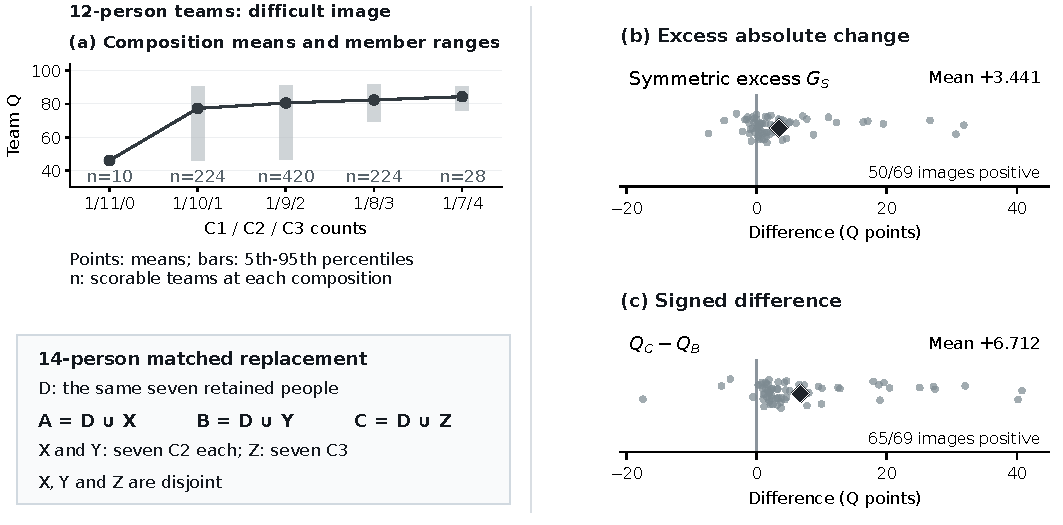
\includegraphics[width=145mm]{figures/composition_replacement_rev11.pdf}
\caption{Composition summaries and specified replacements reveal different aspects of member sensitivity. (a) Twelve-person teams on zsNo4HB9uLZ-16 combine six fixed members with six of twelve candidates. Horizontal labels give C1/C2/C3 member counts; points are mean Q, bars show fifth--95th percentiles, and $n$ gives the number of scorable teams. (b--c) A separate 14-person A--B--C comparison shares seven retained members and exchanges seven-person blocks. (b) Excess magnitude $G_S$ compares cross-profile and within-profile Q changes; (c) signed $Q_C-Q_B$ shows whether C scores higher or lower than B. Each dot is an image mean; diamonds average the 69 image means from 146 scorable events (comparison definitions and supporting results in Supplements C17 and C19).}
\label{fig:composition-members}
\label{fig:matched-half}
\label{fig:team-comparison-design}
\end{figure*}

Across 231 panels (40 panoramas in 22 buildings), we enumerate all 924 ways to select six of twelve candidates and combine them with a background fixed within each panel. Backgrounds contain 6--23 people, producing teams of 12--29; Figure~\ref{fig:composition-members} illustrates a 12-person panel. This enumeration quantifies the balance between profile composition and member choice: under the C1--C3 profile partition, differences between profile compositions account for 15.43\% of the total $Q$ variance, whereas differences among specific member sets within the same composition account for the remaining 84.57\% (weighted by scorable teams within compositions and equally across buildings; Supplement C17). Profile proportions describe mean trends, while member combinations within the same proportions account for most of the variation in these enumerated teams.

Different profile families also expose distinct quality--labor trade-offs. On their respective shared supports in 12-person teams, the one-seat C2-to-C3 composition contrast raises mean $Q$ by 1.963 points with a recorded labor ratio of 1.020 across 27 panoramas. The corresponding J3-to-J4 contrast (ordered by increasing training-fold $Q$ residuals) raises mean $Q$ by 2.701 points with a labor ratio of 0.897 across 14 panoramas. Similarly, historical consensus-response profiles (R1--R2) directly track individual impact on group geometry: R2 annotators outscore R1 annotators by 13.937 individual-$Q$ points across 192 shared panoramas, and cross-profile swaps between R1 and R2 induce larger consensus shifts than within-profile swaps on 62 of 83 panoramas (Supplement C19).

\subsubsection{Within-profile and cross-profile replacements}

Controlled block replacements reveal both the greater magnitude of cross-profile changes and their quality direction: C2-to-C3 exchanges usually raise $Q$, while matched within-profile alternatives establish how much change also occurs when the class is held fixed. In direct A--C comparisons on 14-person teams, replacing a seven-person C2 block with a C3 block (while holding the seven background members fixed) increases team $Q$ by an average of 6.190 points, with positive gains on 77 of 83 panoramas. Adding a matched within-profile control block $B$ in our A--B--C design---where teams $A$ and $B$ add disjoint C2 blocks and team $C$ adds a C3 block to the same seven-person background---shows that cross-profile replacement exceeds within-profile variation by a mean symmetric excess of $G_S = 3.441$ points across 69 jointly scorable panoramas (positive on 50), with team $C$ outscoring team $B$ by $\Delta_{CB} = 6.712$ points (positive on 65; Figure~\ref{fig:matched-half}).

The six-person C1--C3 comparisons sharpen this distinction: cross-profile exchanges produce larger changes in both directions, while reversing the exchange reverses the mean quality effect. In six-person teams, exchanging three members between C1 and C3 across 36 shared panoramas yields mean excess magnitudes of $G_S = 3.269$ (C1-to-C3) and $3.955$ (C3-to-C1), accompanied by signed effects of $\Delta_{CB} = +7.327$ and $-7.777$ $Q$ points, respectively (Supplement C19). In 20-person teams, a seven-person C2-to-C3 replacement increases $Q$ by 4.484 points across 84 panoramas; on the 40 panoramas with shared quality and timing records, $Q$ rises by 4.406 points while total team labor increases by 121.05 person-seconds.

Combining entire profile classes into whole-profile mixtures reveals how incoming votes can either recover missed features or dilute intricate detail. Across 154 shared panoramas in 22 buildings, pooling all available C2 and C3 annotators (C2+C3) expands the team as well as changing its composition, yielding a mean $Q$ of 88.52---outperforming pure C2 teams (84.83) but falling below pure C3 teams (92.29; Figure~\ref{fig:profile-mixtures}). The dilution is sharpest on complex geometry: across 34 difficult panoramas, the C2+C3 mixture scores 19.768 points below pure C3 (losing on 26 panoramas), and across 36 self-occluded panoramas it retains 2.389 fewer turns and 1.389 fewer short edges, alongside an 18.467-point drop in $Q$. When incoming members omit a fine wall turn, their addition can raise the at-least-half threshold beyond its existing support, removing a recess retained by the smaller team (as illustrated in Figure~\ref{fig:bathroom-turn-votes}).

\begin{figure}[t]
\centering
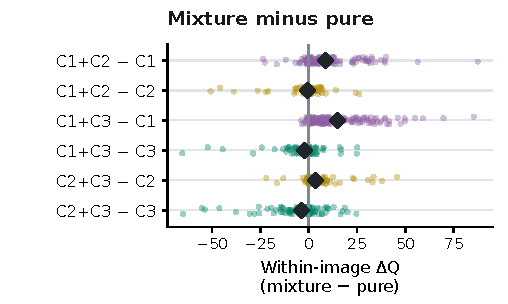
\includegraphics[width=86mm]{figures/profile_mixtures_rev11.pdf}
\caption{Whole-profile mixtures gain relative to one constituent and lose relative to another. Dots are paired image-level mixture-minus-pure Q differences on 154 common images; diamonds are means. Each selected profile contributes all its available members.}
\label{fig:profile-mixtures}
\end{figure}

\subsubsection{Retained people alter replacement direction and boundary position}

The impact of a member replacement depends not only on who is swapped, but also on the retained background $D$. In the joint-profile comparison, expanding the retained background reduces the average magnitude of a fixed exchange: holding seven-person replacement blocks constant while increasing total team size from 20 to 28 reduces the mean absolute $Q$ shift by 1.317 points across 76 panoramas (shrinking on 63). More strikingly, rotating the retained background members can reverse the sign of the exact same exchange. Among 276 replacement blocks evaluated across at least two scorable backgrounds, 56 blocks (20.3\%, spanning seven panoramas) produced both positive and negative $Q$ shifts, with 24 blocks crossing both $+1$ and $-1$ $Q$ points. Even when holding the background's profile counts strictly fixed, 18 of 120 subgroups reversed direction, including nine that crossed both $\pm 1$-point thresholds (Supplement C19).

A concrete 14-person comparison on panorama \texttt{q9vSo1VnCiC-30} illustrates how specific retained members dictate the effect of incoming observations. Two distinct seven-person backgrounds each contained exactly one C1 and six C2 annotators; yet applying the identical seven-person C2-to-C3 replacement reduced $Q$ from 85.130 to 81.090 under the first background while boosting $Q$ from 38.146 to 87.269 under the second, because the two backgrounds anchored the consensus around different initial structures and boundary positions.

Furthermore, member replacements reshape boundary localization even when the corner count remains unchanged; the illustrated case also preserves the corner identities and their ring order. Among 1,829 jointly scorable 20-person replacement pairs, 1,632 retained the exact same number of corners, yet 127 of those constant-count pairs shifted by more than 10 $Q$ points. In panorama \texttt{7y3sRwLe3Va-13} (Figure~\ref{fig:localization-mechanism}), all four room corners retain unanimous 20-vote support and identical cyclic ordering before and after a seven-person swap, yet the new members' endpoint coordinates shift the median consensus positions enough to raise $Q$ from 77.41 to 92.58.

\begin{figure*}[t]
\centering
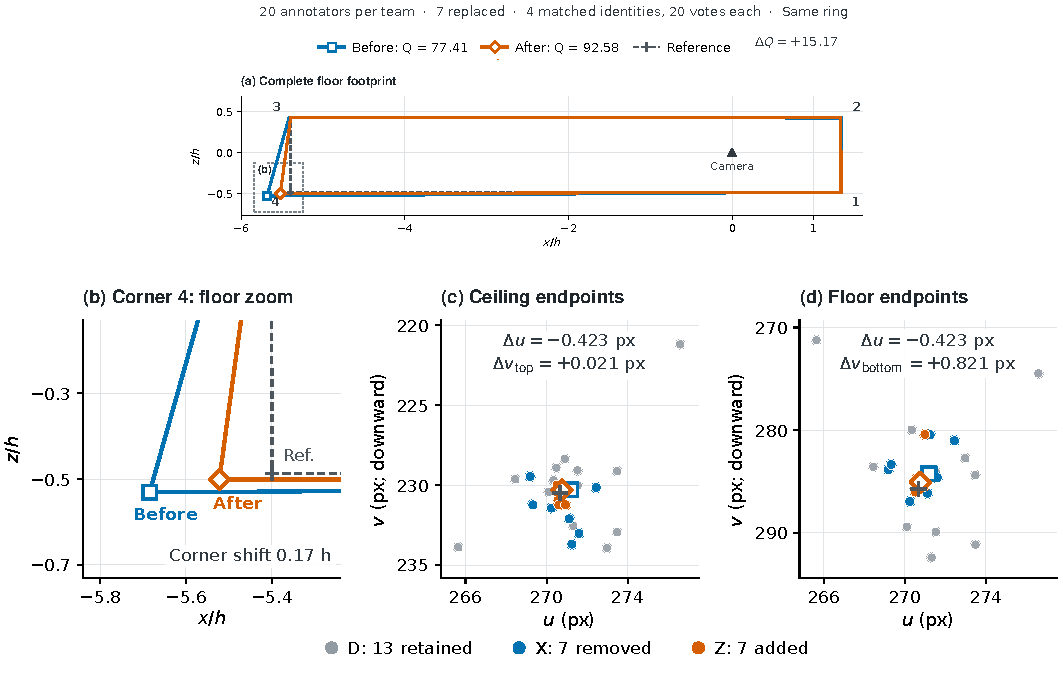
\includegraphics[width=115mm]{figures/localization_compact2.pdf}
\caption{Seven replacements change localization while four identities retain twenty votes and the same ring order in 7y3sRwLe3Va-13. Panels show the complete footprints, corner-4 detail and its upper/lower observations. Gray marks thirteen retained people, blue seven removed and orange seven added; outlined markers are consensus positions. Changes of about 0.42 horizontal and 0.82 lower-endpoint pixels correspond to a floor displacement of $0.17h$ in the 1024 by 512 panorama. Q measures the complete layout.}
\label{fig:localization-mechanism}
\end{figure*}

Decomposing $Q$ into its five geometric components further explains why 7 of 84 panoramas in the 20-person C2-to-C3 exchange gained prism IoU while losing $Q$: on \texttt{x8F5xyUWy9e-03}, for example, $Q$ dropped by 4.726 points as internal directional error rose by $0.836^\circ$ alongside local boundary and height shifts (Supplement C19).



\subsection{Cross-View Repetition, Transfer, and Task Conditions}
\label{sec:viewpoint-scope}
\subsubsection{Structural habits recur while local corner choices change}

When annotators observe the same room from multiple camera viewpoints, their macro-level tendency to retain or simplify architectural structure persists, even as their micro-level decisions at individual corners shift with the camera angle. Across 128 directly paired viewpoints spanning 65 panoramas in 13 buildings, two annotations by the same person differed by an average of 0.671 effective turns, compared to 0.752 turns for pairs drawn from different annotators in the shared worker pool. This individual consistency is most pronounced when both viewpoints contain short reference edges: across 15 such view pairs in five buildings, same-person simplification agreement surpassed the different-person baseline by 13.38 percentage points (73.29\% versus 59.91\%; Table~\ref{tab:same-room-evidence}), yielding a 12.39-point advantage under equal building weighting that held across all five buildings.

\begin{figure*}[t]
\centering
\setcounter{subfigure}{0}
\begin{minipage}{150mm}
\centering
\ESPanel{.3592\linewidth}{panels/fig14/a.pdf}{View 07}%
\hfill%
\ESPanel{.3424\linewidth}{panels/fig14/b.pdf}{View 10}%
\hfill%
\ESPanel{.2684\linewidth}{panels/fig14/c.pdf}{Personal repetition}

\par\vspace{2pt}
\includegraphics[width=.55\linewidth]{\FigureAssetRoot/panels/fig14/legend.pdf}
\par\vspace{2pt}

\end{minipage}
\caption{Two annotators repeat their broader structural habits across views while changing individual corner choices. (a--b) A40 and A41's complete layouts on VFuaQ6m2Qom-07 and -10, with the same narrow-wall endpoints enlarged. Counts are effective/reference turns; dashed lines mark reference azimuths. A40 marks both endpoints in both views. A41 marks neither in view 07 and both in view 10, while simplifying both layouts. (c) Same-person and different-person simplification agreement over fifteen view pairs in five buildings.}
\label{fig:same-room-structure}
\end{figure*}


Same-room case comparisons illustrate how stable global habits coexist with view-dependent local choices. Across four viewpoints of the same room, annotator A40 consistently matched the full reference turn count, whereas annotator A41 simplified the room in every view; yet between views \texttt{VFuaQ6m2Qom-07} and \texttt{-10}, A41 switched from omitting both endpoints of a narrow wall segment to marking both (Figure~\ref{fig:same-room-structure}), and 7 of the 18 shared annotators changed whether they marked the door-side endpoint. Likewise, in a second room spanning three view pairs, 19 of 33, 12 of 30, and 14 of 30 annotators altered their local corner markings across viewpoints, showing how viewpoint-dependent corner choices coexist with recurring tendencies to retain or simplify room structure (Supplement C19).

\subsubsection{Transfer depends on the outcome and the specified people}

Cross-view transfer reflects this contrast between recurring structural expression and view-dependent positions: source-view histories improve short-detail and quality prediction, whereas directly transferring personal pixel offsets increases error. Across 1,793 target annotations (65 panoramas, 56 annotators, 13 buildings), incorporating an annotator's source-view history from the same room reduced short-edge count MAE by 10.4\% relative to source-view peer averages (from 0.526 to 0.472 edges; Table~\ref{tab:same-room-evidence}), an improvement that remained positive under equal building weighting after omitting any one building. Similarly, observing the source-view mean $Q$ lowered target-image mean $Q$ prediction error from 9.496 to 6.464 points and reduced individual $Q$ MAE from 15.645 to 13.385 points when combined with personal history. Conversely, directly transferring an annotator's personal floor-endpoint pixel offset across viewpoints degraded localization, raising MAE from 2.610 to 3.082 pixels, and appending coarse room-use labels to geometric features slightly increased $Q$ MAE from 5.158 to 5.379 points across 190 panoramas.

\begin{table}[t]
\centering\small
\caption{Cross-view repetition and transfer. Short-edge-count MAE is in edges; all Q MAEs are in Q points. Short-edge and individual-Q prediction use 1,793 annotations in thirteen buildings; image-mean prediction uses 128 view pairs. The final row uses reference-derived geometry features. Other supports are shown by row. Protocols and results appear in Supplements C7 and C19.}
\label{tab:same-room-evidence}
\setlength{\tabcolsep}{3pt}
\begin{tabular}{@{}p{.65\linewidth}r@{}}
\toprule
Comparison & Result\\
\midrule
Simplification agreement, same/different person (15 pairs, 5 buildings) & 73.29/59.91\%\\
Short-edge-count MAE, personal history/peers & 0.472/0.526\\
Image-mean Q MAE, source view/external baseline & 6.464/9.496\\
Individual Q MAE, room + personal history/personal history & 13.385/15.645\\
Replacement positive at both views (19 pairs, 7 buildings) & 18/19\\
Composition correlation (127 pairs, 13 buildings) & $-$0.052\\
Q MAE, geometry + room use/geometry (190 images, 21 buildings) & 5.379/5.158\\
\bottomrule
\end{tabular}
\end{table}

At the team level, targeted member replacements transfer robustly across viewpoints, whereas full composition patterns show little cross-view association. In 10-person matched A--B--C comparisons that held five background members fixed and reused each annotator's view-specific submission, replacing five C2 annotators with five C3 annotators increased mean $Q$ in both viewpoints across 18 of 19 room pairs (with 318 of 322 replacement events scorable across all six outputs; Supplement C14). In contrast, broad composition-level performance exhibited a pooled cross-view correlation of $-0.052$ across 127 view pairs, and raw individual $Q$ correlation across views ($0.401$) dropped to $0.013$ after controlling for peer averages and out-of-building personal history. Room-level quality baselines and individual structural histories carry useful information across views, and the specified C2-to-C3 replacements usually retain a positive direction. Full-composition quality shows little cross-view association.

\subsubsection{Doorway targets change closure and group-size responses}
\label{sec:doorway}

We examine doorway-boundary viewpoints as a distinct annotation scene: the camera stands beneath the doorframe between adjoining spaces, exposing more than one plausible enclosure (Figure~\ref{fig:doorway-scene}). Choosing one room or the combined space changes where a layout closes, even when each answer traces a coherent boundary.
\begin{figure*}[t]
\centering
\setcounter{subfigure}{0}
\begin{minipage}{155mm}
\centering
\ESPanel{.44\linewidth}{panels/fig15/original_model_clean.pdf}{Camera beneath the lintel}%
\hfill%
\ESPanel{.54\linewidth}{panels/fig15/b_panorama.pdf}{Panorama at the doorway}

\end{minipage}
\caption{A camera at the doorway boundary. (a) The complete three-dimensional model shows the camera beneath the doorframe and the two adjoining spaces. The external callout locates the camera without covering either room. (b) The actual doorway panorama shows the adjoining spaces visible from this position. The schematic illustrates the spatial arrangement; the panorama provides the scene evidence.}
\label{fig:doorway-scene}
\end{figure*}


When domain experts screened doorway submissions while blinded to $Q$---filtering out degenerate or spatially uninterpretable polygons while retaining coherent enclosures (Supplements B17, B22)---the fixed 17-image panel narrowed from 584 to 439 eligible responses. Evaluated against a common whole-space reference at a team size of 10, screening raised conditional mean $Q$ by 1.581 points and lifted the complete-and-evaluable rate by 7.86 percentage points (Figure~\ref{fig:doorway-screening}a--b).

\begin{figure*}[t]
\centering
\setcounter{subfigure}{0}
\begin{minipage}{140mm}
\centering

\par\vspace{2pt}
\includegraphics[width=.39\linewidth]{\FigureAssetRoot/panels/fig16/legend_ab.pdf}
\par\vspace{2pt}
\ESPanel{.497\linewidth}{panels/fig16/a.pdf}{Whole-space reference: Q (17 images)}%
\hfill%
\ESPanel{.473\linewidth}{panels/fig16/b.pdf}{Whole-space reference: output rate}

\par\vspace{3pt}

\par\vspace{2pt}
\includegraphics[width=.47\linewidth]{\FigureAssetRoot/panels/fig16/legend_cd.pdf}
\par\vspace{2pt}
\ESPanel{.497\linewidth}{panels/fig16/c.pdf}{Assigned targets: Q}%
\hfill%
\ESPanel{.473\linewidth}{panels/fig16/d.pdf}{Assigned targets: output rate}

\end{minipage}
\caption{Doorway screening and target-specific trajectories answer separate questions. (a--b) Screening on the same seventeen images uses a common whole-space reference before and after, at sizes 3--14. (c--d) Assigned-target pools in 7y3sRwLe3Va-18 contain nine people for space 1, four for space 2 and fifteen for the whole space. These pools differ in members and references. Q uses scorable outputs; completion rates use all attempts.}
\label{fig:doorway-screening}
\end{figure*}


In the screened doorway pools containing competing targets, conditional mean $Q$ rose from 38.111 at size 3 to 44.953 at size 6, but plateaued at 44.294 by size 14 (falling by 0.54 points across paths jointly scorable at sizes 6 and 14, with 7 panoramas improving and 10 declining), while completion dipped from 86.63\% to 80.79\% before rebounding to 92.72\%. Partitioning a doorway pool by the specific room enclosure each annotator targeted---such as panorama \texttt{7y3sRwLe3Va-18}, where 28 of 29 screened submissions cleanly separate into nine annotators tracing Space 1, four tracing Space 2, and fifteen tracing the combined space (Figure~\ref{fig:doorway-screening}c--d)---reveals distinct group-size trajectories for the intended enclosures, each evaluated with its corresponding members and reference.

\subsubsection{OOS observations identify representation conditions}

Finally, out-of-scope (OOS) scenes reveal where a single-level Manhattan layout cannot capture the observed architecture. Across 1,222 diagnostic submissions on 28 panoramas, floor structure and upper geometry present distinct representational demands: all 80 Manual submissions on three sloped-ceiling panoramas retained four floor corners, while the ceiling geometry requires height variation. A continuous turning glass boundary presents a different challenge: across five views of the same room, 61.8\% of two-response comparisons differed in corner count, averaged equally over images. Together, the panorama and reconstruction examples connect these patterns to oblique walls, sloping ceilings and changes in floor or ceiling level (Supplement B19).


\section{Discussion}
\label{sec:discussion}

\subsection{Staffing for quality, stability and structure}
Our findings demonstrate that team size and member selection serve distinct operational goals in 3D layout annotation. Expanding a small team rapidly boosts average geometric quality, whereas adding annotators to an already moderate-sized team primarily improves lower-tail quality and narrows between-team variance. However, on visually complex or occluded scenes, aggregate group-size curves mask opposing structural shifts as contested wall turns cross or fall below the at-least-half support threshold. When target disagreement or omission of difficult structures persists, adding more annotators may offer limited benefit; expert assistance can help clarify the target or review the relevant structures.

At the level of team composition, out-of-building profiles capture persistent individual habits, while the existing team context governs how new submissions reshape the consensus layout. Mixing simplifying and turn-retaining profiles can either supply missing wall turns or dilute support for fine architectural recesses below the retention threshold; even when the consensus corner count is unchanged, swapping members shifts boundary localization through the median coordinate estimator. Structural profiles describe individual tendencies, while incoming and retained observations jointly determine which turns are recovered or lost and how boundaries shift.

\subsection{Using observations for annotation support and reference review}
Pairing discrete corner-support records with multi-component geometric measurements ($Q$) provides an interpretable diagnostic framework for dataset curation and reference auditing. Support records trace exactly which annotators contributed to each wall turn and how tightly their clicked endpoints cluster, while the components of $Q$ separate floor-extent errors from boundary displacements, non-orthogonal walls, and local ceiling distortions. Consequently, whenever a visible wall turn receives strong multi-annotator support yet is absent from an existing benchmark reference, it surfaces immediately as an actionable candidate for expert reference revision.

The cross-view and task-condition results guide annotation and reference review. Linking multiple viewpoints of the same room allows curation pipelines to cross-check contested corners and transfer individual structural histories, while doorway scenes benefit from explicitly specifying whether the target enclosure terminates at the doorframe or extends into the adjoining space. OOS diagnostics distinguish geometric requirements: oblique walls require relaxing the Manhattan direction assumption, sloped ceilings require varying upper heights, and split-level floors require representing more than one ground plane. Finally, because Semi submissions can retain known initialization errors even after editing, interactive annotation tools should highlight uncertain model boundaries, visualize multi-annotator support and coordinate spread, and link 2D panorama clicks directly to 3D wall previews.

\subsection{Quality and recorded labor in offline policies}
\label{sec:labor-history}

Existing histories support lower target labor in the selection comparison, while acquiring histories changes the cost of adaptive stopping. At team size five, quality-and-time selection has mean $Q=93.926$ versus $93.708$ for historical-$Q$ selection across 126 contexts from 46 images in nine buildings. Their paired difference is $+0.218$ ($95\%$ building-bootstrap CI $[-0.538,0.869]$), and the geometric mean recorded-labor ratio is 0.813 ($[0.760,0.882]$).

Source-history stopping raises mean $Q$ from 85.189 to 86.054 on 21 images in five room groups. Its timing panel contains 11 images in three groups: target labor increases from 1,307.9 to 1,660.3 person-seconds, and including history acquisition gives a project-labor ratio of 2.115. The stopping rule improves observed quality and requires more work. Supplement D reports the full comparisons alongside Supplements C9, C13 and C14.



\section{Conclusion}

We present a framework for studying how individual panoramic layout observations become collective geometry. It combines geometric quality measurement, paired-corner structural consensus and controlled team comparisons under explicit target-space definitions. $Q$ measures extent, boundary, direction and height discrepancies; consensus carries distinct-person support and local upper--lower observations into a connected layout. Controlled geometry and human defect reports support the interpretation of $Q$. Shared-team traces show how supported turns and upper endpoints enter consensus. Doorway-boundary viewpoints identify a setting in which camera position makes the target enclosure a separate decision.

The four research questions reveal complementary sources of variation. People differ in retained structure and boundary placement. Adding people changes the mean, lower tail and variability at different rates. Profile composition, specific members and retained background jointly determine which turns survive and where boundaries fall. Structural habits recur across views, while local choices and quality transfer depend on the observed scene. These findings connect team organization and targeted reference review to the structures and positions that annotation datasets actually contain.


\FloatBarrier
\section*{Data and code availability}
Supplementary files provide method source snapshots, controlled-geometry inputs, analysis tables, and anonymized questionnaire answers with display mapping. Scripts reproduce questionnaire summaries and saved-effect aggregates; the implementation guide specifies the full geometry and fusion pipeline's inputs and dependencies.

\setlength{\bibsep}{2pt plus 1pt minus 1pt}
\begin{thebibliography}{00}
\bibitem{chang2017matterport3d} Chang, A. X., et al. (2017). Matterport3D: Learning from RGB-D data in indoor environments. Proceedings of the International Conference on 3D Vision.
\bibitem{zou2021manhattan} Zou, C., Su, J.-W., Peng, C.-H., Colburn, A., Shan, Q., Wonka, P., Chu, H.-K., \& Hoiem, D. (2021). Manhattan Room Layout Reconstruction from a Single 360$^\circ$ Image: A Comparative Study of State-of-the-Art Methods. International Journal of Computer Vision, 129(5), 1410--1431. DOI: 10.1007/s11263-020-01426-8.
\bibitem{c2ref06} Tsai, Y.-J., Jhang, J.-C., Zheng, J., Wang, W., Chen, A. Y. C., Sun, M., Kuo, C.-H., \& Yang, M.-H. (2024). No More Ambiguity in 360$^\circ$ Room Layout via Bi-Layout Estimation. Proceedings of the IEEE/CVF Conference on Computer Vision and Pattern Recognition (CVPR), 28056--28065.
\bibitem{pano2018} Yang, S.-T., Peng, C.-H., Wonka, P., \& Chu, H.-K. (2018). PanoAnnotator: A Semi-Automatic Tool for Indoor Panorama Layout Annotation. SIGGRAPH Asia 2018 Posters. DOI: 10.1145/3283289.3283304.
\bibitem{lee2018} Lee, D. J.-L., Das Sarma, A., \& Parameswaran, A. (2018). Aggregating Crowdsourced Image Segmentations. HCOMP 2018 Works in Progress and Demonstration Papers, CEUR Workshop Proceedings, Vol. 2173.
\bibitem{c2ref01} Zhang, Y., Song, S., Tan, P., \& Xiao, J. (2014). PanoContext: A Whole-room 3D Context Model for Panoramic Scene Understanding. In European Conference on Computer Vision (ECCV), 668--686. DOI: 10.1007/978-3-319-10599-4\_43.
\bibitem{horizon2019} Sun, C., Hsiao, C.-W., Sun, M., \& Chen, H.-T. (2019). HorizonNet: Learning Room Layout With 1D Representation and Pano Stretch Data Augmentation. Proceedings of the IEEE/CVF Conference on Computer Vision and Pattern Recognition (CVPR), 1047--1056.
\bibitem{cruz2021zind} Cruz, S., Hutchcroft, W., Li, Y., Khosravan, N., Boyadzhiev, I., \& Kang, S. B. (2021). Zillow Indoor Dataset: Annotated Floor Plans With 360$^\circ$ Panoramas and 3D Room Layouts. Proceedings of the IEEE/CVF Conference on Computer Vision and Pattern Recognition (CVPR), 2133--2143. DOI: 10.1109/CVPR46437.2021.00217.
\bibitem{dong2024panocontext} Dong, Y., Fang, C., Bo, L., Dong, Z., \& Tan, P. (2024). PanoContext-Former: Panoramic Total Scene Understanding with a Transformer. Proceedings of the IEEE/CVF Conference on Computer Vision and Pattern Recognition (CVPR), 28087--28097. Supplementary Material, Section 1.
\bibitem{kanayama2025tof360} Kanayama, H., Chamseddine, M., Guttikonda, S., Okumura, S., Yokota, S., Stricker, D., \& Rambach, J. (2025). ToF-360: A Panoramic Time-of-Flight RGB-D Dataset for Single Capture Indoor Semantic 3D Reconstruction. Proceedings of the IEEE/CVF Conference on Computer Vision and Pattern Recognition Workshops, 4481--4490.
\bibitem{horizoneval} Sun, C., Hsiao, C.-W., Sun, M., \& Chen, H.-T. HorizonNet general-layout evaluation (\texttt{eval\_general.py}). Software accompanying HorizonNet, CVPR 2019. \url{https://github.com/sunset1995/HorizonNet/blob/master/eval_general.py}. Accessed 10 November 2026.
\bibitem{c2ref13} Dawid, A. P., \& Skene, A. M. (1979). Maximum Likelihood Estimation of Observer Error-Rates Using the EM Algorithm. Journal of the Royal Statistical Society: Series C (Applied Statistics), 28(1), 20--28. DOI: 10.2307/2346806.
\bibitem{c2ref08} Welinder, P., Branson, S., Belongie, S. J., \& Perona, P. (2010). The Multidimensional Wisdom of Crowds. Advances in Neural Information Processing Systems, 23.
\bibitem{c2ref09} Yan, Y., Rosales, R., Fung, G., Schmidt, M., Hermosillo, G., Bogoni, L., Moy, L., \& Dy, J. (2010). Modeling Annotator Expertise: Learning When Everybody Knows a Bit of Something. Proceedings of the Thirteenth International Conference on Artificial Intelligence and Statistics (AISTATS), PMLR 9, 932--939.
\bibitem{c2ref07} Kairam, S., \& Heer, J. (2016). Parting Crowds: Characterizing Divergent Interpretations in Crowdsourced Annotation Tasks. Proceedings of the ACM Conference on Computer-Supported Cooperative Work \& Social Computing (CSCW), 1635--1646. DOI: 10.1145/2818048.2820016.
\bibitem{c2ref10} Pavlick, E., \& Kwiatkowski, T. (2019). Inherent Disagreements in Human Textual Inferences. Transactions of the Association for Computational Linguistics, 7, 677--694. DOI: 10.1162/tacl\_a\_00293.
\bibitem{c2ref11} Dumitrache, A., Inel, O., Timmermans, B., Ortiz, C., Sips, R.-J., Aroyo, L., \& Welty, C. (2021). Empirical Methodology for Crowdsourcing Ground Truth. Semantic Web, 12(3), 403--421. DOI: 10.3233/SW-200415.
\bibitem{c2ref19} Sheng, V. S., Provost, F. J., \& Ipeirotis, P. G. (2008). Get Another Label? Improving Data Quality and Data Mining Using Multiple, Noisy Labelers. Proceedings of the 14th ACM SIGKDD International Conference on Knowledge Discovery and Data Mining (KDD), 614--622. DOI: 10.1145/1401890.1401965.
\bibitem{c2ref14} Warfield, S. K., Zou, K. H., \& Wells, W. M. (2004). Simultaneous Truth and Performance Level Estimation (STAPLE): An Algorithm for the Validation of Image Segmentation. IEEE Transactions on Medical Imaging, 23(7), 903--921. DOI: 10.1109/TMI.2004.828354.
\bibitem{c2ref17} Braylan, A., Marabella, M., Alonso, O., \& Lease, M. (2023). A General Model for Aggregating Annotations Across Simple, Complex, and Multi-Object Annotation Tasks. Journal of Artificial Intelligence Research, 78, 901--973. DOI: 10.1613/jair.1.14388.
\bibitem{c2ref21} Pradhan, V. K., Schaekermann, M., \& Lease, M. (2022). In Search of Ambiguity: A Three-Stage Workflow Design to Clarify Annotation Guidelines for Crowd Workers. Frontiers in Artificial Intelligence, 5, 828187. DOI: 10.3389/frai.2022.828187.
\bibitem{c2ref12} Gurari, D., Sameki, M., \& Betke, M. (2016). Investigating the Influence of Data Familiarity to Improve the Design of a Crowdsourcing Image Annotation System. Proceedings of the AAAI Conference on Human Computation and Crowdsourcing (HCOMP), 4(1), 59--68. DOI: 10.1609/hcomp.v4i1.13294.
\bibitem{c2ref23} Wang, H., Hutchcroft, W., Li, Y., Wan, Z., Boyadzhiev, I., Tian, Y., \& Kang, S. B. (2022). PSMNet: Position-Aware Stereo Merging Network for Room Layout Estimation. Proceedings of the IEEE/CVF Conference on Computer Vision and Pattern Recognition (CVPR), 8616--8625.
\bibitem{c2ref24} Solarte, B., Wu, C.-H., Liu, Y.-C., Tsai, Y.-H., \& Sun, M. (2022). 360-MLC: Multi-view Layout Consistency for Self-training and Hyper-parameter Tuning. Advances in Neural Information Processing Systems (NeurIPS), 35.
\bibitem{c2ref25} Snow, R., O'Connor, B., Jurafsky, D., \& Ng, A. Y. (2008). Cheap and Fast---but Is It Good? Evaluating Non-Expert Annotations for Natural Language Tasks. Proceedings of the 2008 Conference on Empirical Methods in Natural Language Processing (EMNLP), 254--263. DOI: 10.3115/1613715.1613751.
\bibitem{hohonet2021} Sun, C., Sun, M., \& Chen, H.-T. (2021). HoHoNet: 360 Indoor Holistic Understanding With Latent Horizontal Features. Proceedings of the IEEE/CVF Conference on Computer Vision and Pattern Recognition (CVPR), 2573--2582.
\bibitem{plank2022variation} Plank, B. (2022). The ``Problem'' of Human Label Variation: On Ground Truth in Data, Modeling and Evaluation. Proceedings of the 2022 Conference on Empirical Methods in Natural Language Processing, 10671--10682. DOI: 10.18653/v1/2022.emnlp-main.731.
\bibitem{levy2021suggestions} Levy, A., Agrawal, M., Satyanarayan, A., \& Sontag, D. (2021). Assessing the Impact of Automated Suggestions on Decision Making: Domain Experts Mediate Model Errors but Take Less Initiative. Proceedings of the 2021 CHI Conference on Human Factors in Computing Systems, 1--13. DOI: 10.1145/3411764.3445522.
\end{thebibliography}
\end{document}
